% Created 2020-05-06 mié 14:13
% Intended LaTeX compiler: pdflatex
\documentclass[a4paper, 12pt]{article}
\usepackage[utf8]{inputenc}
\usepackage[T1]{fontenc}
\usepackage{graphicx}
\usepackage{grffile}
\usepackage{longtable}
\usepackage{wrapfig}
\usepackage{rotating}
\usepackage[normalem]{ulem}
\usepackage{amsmath}
\usepackage{textcomp}
\usepackage{amssymb}
\usepackage{capt-of}
\usepackage{hyperref}
\usepackage{float, amsfonts, commath, mathtools, proba}
\author{Tabaré Pérez}
\date{\today}
\title{Lecture 16 - 5: Mixture Model - Unobserved Case: EM Algorithm}
\hypersetup{
 pdfauthor={Tabaré Pérez},
 pdftitle={Lecture 16 - 5: Mixture Model - Unobserved Case: EM Algorithm},
 pdfkeywords={},
 pdfsubject={},
 pdfcreator={Emacs 26.3 (Org mode 9.3.6)}, 
 pdflang={English}}
\begin{document}

\maketitle
From "Lecture 16 - 4: Mixture Model - Observed Case" we have:

\begin{equation}
\label{eq:orgef74bfa}
\hat{n}_j = \sum_{i=1}^{n} \delta(j|i)
\end{equation}

\begin{equation}
\label{eq:org0f5d777}
\hat{\prob}_j = \frac{\hat{n}_j}{n}
\end{equation}

\begin{equation}
\label{eq:orge5b0289}
\hat{\mu}^{(j)} = \frac{1}{\hat{n}_j} \sum_{i=1}^{n} \delta(j|i) x^{(i)}
\end{equation}

\begin{equation}
\label{eq:org524d709}
\hat{\sigma}_{j}^{2} = \frac{1}{\hat{n}_j} \sum_{i=1}^{n} \delta(j|i) \norm{x^{(i)} - \mu^{(j)}}^2
\end{equation}

So the next question that we need to answer is, how can we do it if we actually
don't have at all information about the identity of the points?

So before I start describing to you how can we do it formally, I want to give
you an intuition how it would go. So what did we do here?

The reason we introduced this notation, this \(\delta(j|i)\) it's actually a hard count:
The point either belongs here, or it doesn't belong, it was \(0\) or \(1\).

Now, one of the powers of our mixture model, that actually model doesn't solely
belong to this cluster, we know that it can be generated from different ones
with different probabilities.

So now, instead of talking about hard counts belong or doesn't, we're actually
talking about soft counts. How much does this point belongs to this particular
cluster?

But when I just give you this spread of wide points, I don't know how much does
it belong to the cluster, because I don't have the parameters.

You agree with me that if I will actually specify to you all the parameters that
we need to know, all the \(\mu\)s and the \(\sigma^2\) and the \(\prob\), you
can actually answer this question.

You can say, how much does it belong to one cluster versus another cluster. But
you don't have it.

You don't know. it's kind of chicken and egg problem because you don't know
where it belongs, but you also don't know the parameters.

So what we are going to be doing here, we're actually going to break it down,
and intuitively speaking, what we will do we will say I randomly guess the
parameters. I randomly selected the \(\prob\)'s, and I randomly selected the
\(\mu\)s, and I randomly selected the \(\sigma^2\) for each one of those
components. We can later discuss what does it mean randomly selected and what
the implications of it.

For now, just say you magically come up with some things which may not
necessarily be the perfect one, but you come up. This is your first estimate.

And in your head, you should be thinking about K-means clustering. You remember,
when we started talking there, we just randomly selected the representative of
each cluster. We randomly selected them. So here, we selected randomly a bit
more than that. We're not only selecting the \(\mu\)s, but we're also selecting
the \(\sigma^2\), and we're also selecting the mixture weights, the \(\prob\)s.
So I selected them.

Now what happens?: Now I can actually compute the soft counts. For each point, I
can say how likely that this point actually belongs to this cluster. This will
be a soft equivalent of this measure:

\begin{itemize}
\item Here, I just say, is point \(i\) assigned to cluster \(j\)?
\item Now we say, how likely is it that the point \(i\) comes from the cluster
\(j\)?
\end{itemize}

So it's going to be 0 and 1, it could be some other number.

But what it actually means is that instead of using \(\delta(j|i)\), I can use
here the probability: the point is assigned.

So as previously, when I did all this computation, instead of taking this
indicator function \(0\) and \(1\)s, I'm just going to be using probability.

And I will do exactly the same computations. So what would happen here that
after I made these guesses, I can compute this soft assignment of points to
clusters.

And what will be the next natural step?

Now that the points belong to the cluster, I guess I should go back and
recompute the parameters, again, maximizing my likelihood of observed data. And
once I recomputed the parameters, hopefully in a better way, which maximizes the
likelihood,

I can now go and reassess the soft counts. And I can continue these two steps.
And so the first step is the expectation. It's called \textbf{Expectation-Maximization}.

The first one, we are computing the likelihood that the point belongs to a
certain mixture component, and then we maximize the likelihood by assessing the
parameters. And we can continue doing these two steps until there is no change
in our parameters, or they're close enough.

So, for now, let's assume that we know how to do initialization, and I will talk
about it later, and let's just focus on these two steps.

So the first step, the expectation step \textbf{E} and the maximization step \textbf{M}. There
are two steps that we're going to address. And in your head, you can think about
K-means clustering, which would be very much a hard version of the same idea.

And to make it more visual for you, I want you to look at this slide:

\begin{figure}[H]
\centering
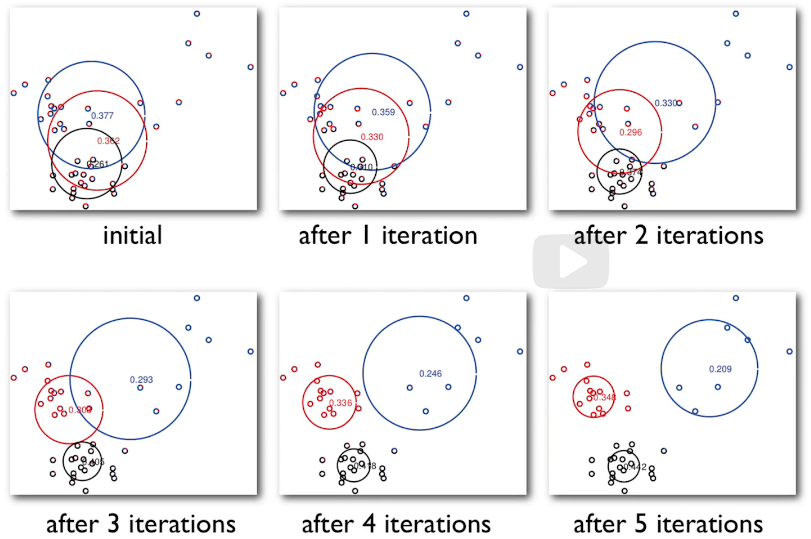
\includegraphics[width=0.8\textwidth]{./pic/u04-05-fig-01.png}
\caption{\label{fig:org5d6dd08}EM Algorithm}
\end{figure}

You see the points after I randomly guessed these parameters and now, if you
look at the points, you would see that the points are colored in multiple colors
you can see that we have a red and a blue, and maybe some points are more
belonging to the red cluster and some are more belonging to the blue cluster and
so on. And you can see that as we do the estimation, the red and blue and other
colors move around. And then the coloring of each point, it's kind of allegiance
to different mixture components changes, and we continue going through these
steps until we come to the convergence.

So it's graphically very easy to see.
But let me now go back to formal description.

And what I will try by first introducing you some notation, which is very
expected notations. And then we will very much reuse this language to do one of
the step of the algorithms. So again, the zero step for us again:

\begin{itemize}
\item E-step, zero step, we randomly initialize all the \(\theta\)s:
\end{itemize}
\begin{equation}
\label{eq:org0264e7d}
\theta; \mu^{(1)} \ldots \mu^{(K)}, \sigma_{1}^{2} \ldots \sigma_{K}^{2}, \prob_1 \ldots \prob_K
\end{equation}

Next, the first step that we are going to do is called \textbf{E step}.
This is a step that your goal for each point
is say exactly the same equation as you've
done before.
What is the likelihood that my point \(i\) belong to cluster \(j\)?
And we will use posteriors to make this assessment:

\begin{itemize}
\item E-step first step:
\end{itemize}
\begin{equation}
\label{eq:orga68cc82}
\prob(j|i) = \frac{\prob_j \mathcal{N}(x^{(i)}; \mu^{(j)}, \sigma_{j}^2 I)}{\prob(x|\theta)}
\end{equation}

And we can do, for the estimation, you remember, we look how we can actually
compute the likelihood of \(x\) being generated by our mixture. It is going to
be some of this expression along all the mixture components. I would not write
it down, but you can quite imagine what we do. We would take this over all
possible \(j\)'s from \(1\) to \(K\) and sum them up. So the point that I'm
trying to make is that after I find, after I give you these numbers, you can
make this computation. So this is pretty straightforward and this is the place,
if you remember the pictures that I showed you, this is a place that would allow
you to say how much red versus blue versus black the point has, because the
coloring at that point would be proportional to its likelihood to be of the red
cluster. Now comes the next step.

So great. Now you have all your points, and we know how much of red or blue or
black color. And what I want to do, I want to re-estimate my parameters to make
them more consistent with the current assignment of the soft counts. So this is
a step when I want to recompute the \(\prob_j\), the \(\mu^{(j)}\), and the
variance for cluster \(j\). That's what I want to do.

So how can we do it? Let's think how the computation changes when we, instead of
using our \(\delta\)s, we're going to be using probabilities, because they
reflect our soft counts. So let's start with the first point. How do we compute
here \(\hat{n}_j\), which is the size of the cluster?

So here, now, when we're talking about the size of the cluster, we will just
take the soft counts, how much the point belongs to this cluster, and sum them
up:

\begin{itemize}
\item M-step first step:
\end{itemize}
\begin{equation}
\label{eq:org1e17bff}
\hat{n}_j = \sum_{i=1}^{n} \prob(j|i)
\end{equation}

We'll go from \(1\) to \(n\) and look at probability of a point to belong to
this cluster.

The next thing that we need to do we need to compute the mixture weight, the
\(\prob\), of cluster \(j\). So what we will do is exactly the same thing. We're
going to take the size of the cluster, which in this case is computed with soft
counts, and divide it by the number of points. So we don't even need to change
the formula:

\begin{itemize}
\item M-step second step:
\end{itemize}
\begin{equation}
\label{eq:org5df7d25}
\hat{\prob}_j = \frac{\hat{n}_j}{n}
\end{equation}

So let's look what happens here. Here, what we've said, the same way we were
inspired by what happened in the real Gaussians, we took the expression that we
had before and just we said, in order to say that the point belonged to the
cluster we used this indicator function. Now, instead of the indicator function,
there's not enough for whether it belongs or it doesn't because it belongs to
everybody with different probabilities. I am just going to weight the point in
the sum according to its likelihood to belong to that cluster. So in this
particular case, again, we can just derive this expression:

\begin{itemize}
\item M-step third step:
\end{itemize}
\begin{equation}
\label{eq:org837258c}
\hat{\mu}^{(j)} = \frac{1}{\hat{n}_j} \sum_{i=1}^{n} \prob(j|i) x^{(i)}
\end{equation}

And in a very similar fashion, you can do the same computation when we are
computing the variance. Again, we're going to substitute here the delta with a
probability:

\begin{itemize}
\item M-step fourth step:
\end{itemize}
\begin{equation}
\label{eq:org71e48f8}
\hat{\sigma}^2 = \frac{1}{\hat{n}_jd} \sum_{i=1}^{n} \prob(j|i) \norm{x^{(i)} - \mu^{(j)}}^2
\end{equation}

Now I have all the parameters that I need after my first step of m. Now I
started with totally random numbers. I did the computation, and now I should
have a better estimate of the parameters. So since I have now the new
parameters, I can go back and recompute the probability of the points to belong
to a certain cluster. And once I complete it, I can go back and forth.

So it will continue this process until convergence. So now I want to emphasize
these numbers, (\ref{eq:org1e17bff}, \ref{eq:org5df7d25}, \ref{eq:org837258c} and \ref{eq:org71e48f8} ) How did they come about?
How, for instance, this number came about? We can actually take, again, our
expression for the likelihood, and because the points are now, we know to which
cluster they belong, we can take the expression for the likelihood, take the
derivative, do the whole computation, and demonstrate that they will have this
specific form.

You don't have to do it, and hopefully you are convinced based on our
conversation. But if you want to, you can go and do the whole computation the
way we've done it in all these other situations, and demonstrate that this will
be the form of these expressions.

And again, the so that you may be thinking, so why I didn't take my original
expression, which is here, just logged it, and just did the derivation directly?
And the reason we didn't do it, because whenever we're taking the log of this
expression, we're getting sum of log of sum, and all these parameters are
intertwined. It's actually really non-trival for us to compute the estimates of
all these variables, because they're very interconnected.

So therefore, we're taking this way, where we are breaking these dependence by
first assuming what are the parameters and computing the likelihoods of points
belonging to different clusters, and then use it to do the computation.

And if you look now at the slide, you can really see how the M and E step
interact, bringing more homogeneous points together and coloring them into the
same color.

So now I want to say another two things related to the guarantees related to E-M
algorithm.

What we can say about E-M algorithm is that it's guaranteed to converge locally,
which means that if we are starting with different random starting points, we
may get very different answer, depending where we start.

And this is actually one of the very weak point of the algorithm, so you really
need to know how to initialize, or you need to have some hunch how to initialize
it, to bring you to a good spot. And you can think, for instance, in our case of
mixture model, what would be a reasonable initialization? So, for instance, what
you can do here, you can just run k-means algorithm and get the \(\mu\)s from k-means
algorithm, which will be your original \(\mu\)s, and then maybe use the global
variance as the variance for each one of the clusters, so that every cluster has
reach of all the points.

And typically what people do in real problems, and EM is really, really widely
used, sometimes people may look at a more simplified version of the problem to
utilize it as initialization to more complex one. And there are lots of
interesting uses of E-M, and I hope that you will explore some of them in your
exercises. Thank you.

\textbf{E-M ALGORITHM SUMMARY}:

\begin{itemize}
\item E-step zero step: we randomly initialize all the \(\theta\)s:
\end{itemize}

\begin{equation}
\theta; \mu^{(1)} \ldots \mu^{(K)}, \sigma_{1}^{2} \ldots \sigma_{K}^{2}, \prob_1 \ldots \prob_K
\end{equation}

\begin{itemize}
\item E-step first step:
\end{itemize}

\begin{equation}
\prob(j|i) = \frac{\prob_j \mathcal{N}(x^{(i)}; \mu^{(j)}, \sigma_{j}^2 I)}{\prob(x|\theta)}
\end{equation}

\begin{itemize}
\item M-step first step:
\end{itemize}

\begin{equation}
\hat{n}_j = \sum_{i=1}^{n} \prob(j|i)
\end{equation}

\begin{itemize}
\item M-step second step:
\end{itemize}

\begin{equation}
\hat{\prob}_j = \frac{\hat{n}_j}{n}
\end{equation}

\begin{itemize}
\item M-step third step:
\end{itemize}

\begin{equation}
\hat{\mu}^{(j)} = \frac{1}{\hat{n}_j} \sum_{i=1}^{n} \prob(j|i) x^{(i)}
\end{equation}

\begin{itemize}
\item M-step fourth step:
\end{itemize}

\begin{equation}
\hat{\sigma}^2 = \frac{1}{\hat{n}_jd} \sum_{i=1}^{n} \prob(j|i) \norm{x^{(i)} - \mu^{(j)}}^2
\end{equation}
\end{document}